\section{Methodology}

\subsection{Data Preparation}
There were two phases attempted during this assignment to aid in understanding. The first set of algorithms used worked with the following data sets: 
\begin{itemize}
    \item Raw Data
    \item PCA 2d
    \item PCA 3d
    \item PCA 4d
    \item PCA 5d
    \item t-SNE 2d
    \item t-SNE 3D
\end{itemize}

Many algorithms were run against these data sets and the results are graphed in the appendix.\par
The second phase of our discovery for this assignment used the following data sets:

\begin{itemize}
    \item Raw Data
    \item PCA 10d
    \item t-SNE 3d
    \item t-SNE 2d
\end{itemize}

We will refer the reader to the Jupyter notebook to align the results of the of the first phase to the graphs in the appendix. The training runs took many hours and were reduced to the following algorithms to increase consistency.\par


\subsection{Active Learning Rare Class Discovery}
For the active learning rare class discovery algorithm, we implemented the following query strategies:
\begin{itemize}
    \item Uncertainty Sampling
    \item Mahalanobis Uncertainty Sampling
    \item Random Sampling
\end{itemize}
These query strategies were stored in the \texttt{strategies} list.

Additionally, we used the following classifier models for the active learning algorithm:
\begin{itemize}
    \item K-Nearest Neighbors with k=10
    \item Random Forest
    \item Support Vector Machine
\end{itemize}
These models were stored in the \texttt{models} list.

\subsection{Visualization}
To gain insights into the structure of the datasets, we visualized the data using 2D and 3D t-SNE projections. The 2D t-SNE plots are shown in Figure~\ref{fig:tsne_2d}, and the 3D t-SNE plots are shown in Figure~\ref{fig:tsne_3d}. The 3D t-SNE visualization is also provided as a MP4 movie to allow for interactive exploration of the data.\par
We also generated an animation of the 3D t-SNE visualization to provide a more interactive and dynamic view of the data. This animation allows for a more detailed exploration of the data, revealing potential clusters and outliers that may not be as apparent in static visualizations.
\begin{figure}[htbp]
\centering
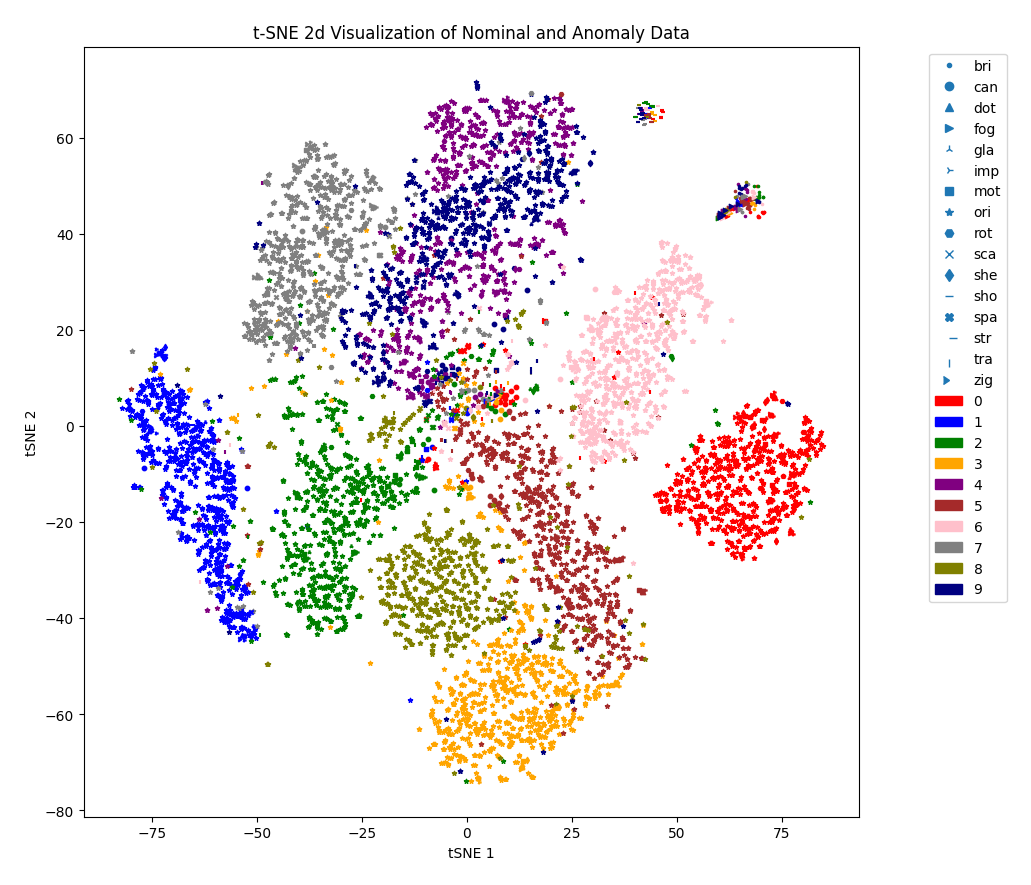
\includegraphics[width=0.5\textwidth]{resources/images/tsne_2d.png}
\caption{2D t-SNE Visualization of the Dataset}
\label{fig:tsne_2d}
\end{figure}

\begin{figure}[htbp]
\centering
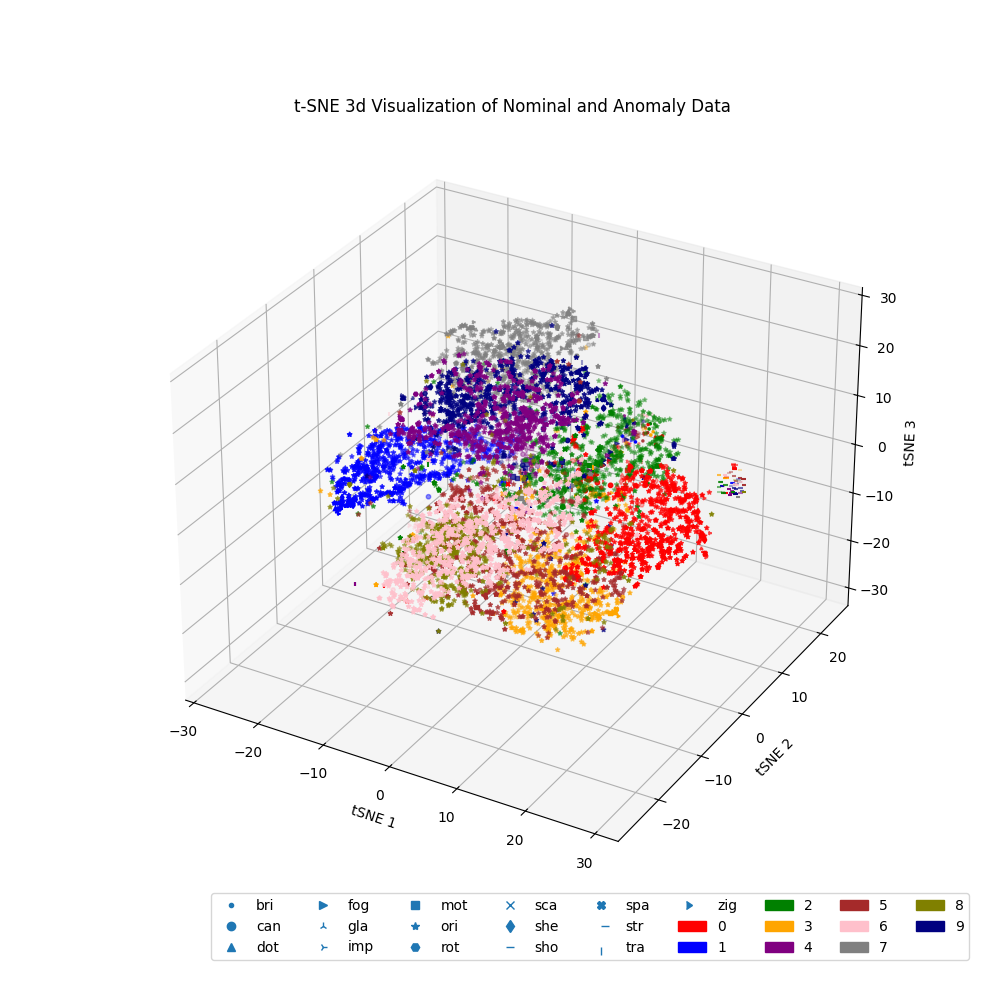
\includegraphics[width=0.5\textwidth]{resources/images/tsne_3d.png}
\caption{3D t-SNE Visualization of the Dataset}
\label{fig:tsne_3d}
\end{figure}